\chapter{Conjugated Carbonyls: Michael and Robinson}\label{ch:b2:conjugate-additions}

The four rings of a steroid hormone were first assembled one ring at a time, and one sequence of
reactions became the standard way of adding a ring: it builds a whole six-membered ring, ketone
included, from a ketone and a small unsaturated ketone. It works because a carbonyl group conjugated
with a \ce{C=C} double bond passes its electrophilic character on to the far end of that double bond.
This chapter is about that far end: which nucleophiles attack it, why, and what can be built with it.

\begin{recall}
\Cref{ch:b2:enolates-aldol}: \omterm{def:b2:enolates-aldol:enolate}{enolates}, the \omterm{def:b2:enolates-aldol:aldol}{aldol condensation}. \Cref{ch:b2:frontier-orbitals}: charge
and \omterm{def:b2:frontier-orbitals:control}{orbital control}, hard and soft reagents. \Cref{ch:b2:huckel}: Hückel orbitals and $\pi$ charges.
The Year 1 volume: Grignard reagents and hydrides, kinetic and thermodynamic control, conjugated
systems.
\end{recall}

\section{Two electrophilic sites}

\begin{definition}[$\alpha,\beta$-Unsaturated carbonyl compounds]\label{def:b2:conjugate-additions:enone}
An \emph{$\alpha,\beta$-unsaturated carbonyl compound}\index{alpha,beta-unsaturated carbonyl compound@$\alpha,\beta$-unsaturated carbonyl compound}
has a \ce{C=C} double bond between the $\alpha$
and $\beta$ carbons of a carbonyl compound, conjugated with the \ce{C=O}: an enone (ketone), an enal
(aldehyde), an unsaturated ester or \omterm{def:b2:amines:nitrile}{nitrile}. The simplest are propenal \ce{CH2=CHCHO} and
but-3-en-2-one \ce{CH2=CHCOCH3} (methyl vinyl ketone).
\end{definition}

\begin{omfigure}
\setchemfig{atom sep=1.9em}
\schemestart
\chemfig{H_2C=CH-CH=O}
\arrow{<->}
\chemfig{H_2C=CH-\chemabove{C}{\scriptstyle +}H-\chemabove{O}{\scriptstyle -}}
\arrow{<->}
\chemfig{\chemabove{C}{\scriptstyle +}H_2-CH=CH-\chemabove{O}{\scriptstyle -}}
\schemestop
\par\medskip

\begin{tikzpicture}
\begin{axis}[ybar, width=0.47\linewidth, height=4.6cm, ymin=-0.6, ymax=0.4,
  xtick={1,2,3,4}, xticklabels={C$\beta$,C$\alpha$,C(O),O}, axis x line=bottom, axis y line=left,
  extra y ticks={0}, extra y tick style={grid=major, grid style={black!50}}, enlarge x limits=0.15,
  tick label style={font=\scriptsize}, ylabel={$\pi$ charge}, label style={font=\small},
  title={\small $\pi$ charges of propenal}, bar width=8pt]
\addplot[fill=omDef!50, draw=omDef] table[x=atom, y=q] {figdata/out/bachelor-2-huckel-d.dat};
\end{axis}
\end{tikzpicture}\hfill
\begin{tikzpicture}
\begin{axis}[ybar, width=0.47\linewidth, height=4.6cm, ymin=-0.8, ymax=0.8,
  xtick={1,2,3,4}, xticklabels={C$\beta$,C$\alpha$,C(O),O}, axis x line=bottom, axis y line=left,
  extra y ticks={0}, extra y tick style={grid=major, grid style={black!50}}, enlarge x limits=0.15,
  tick label style={font=\scriptsize}, ylabel={coefficient}, label style={font=\small},
  title={\small LUMO of propenal}, bar width=8pt]
\addplot[fill=omThm!45, draw=omThm] table[x=atom, y=c] {figdata/out/bachelor-2-huckel-d.dat};
\end{axis}
\end{tikzpicture}

{\small Propenal. Top: its three resonance structures; the last two put a positive charge on the
carbonyl carbon and on the $\beta$ carbon. Bottom: the Hückel model of
\cref{ch:b2:frontier-orbitals} ($\alpha_{\ce{O}} = \alpha + \beta$, $\beta_{\ce{CO}} = \beta$; a model).
The largest positive charge is on the carbonyl carbon (+0.33, against +0.23 on the $\beta$ carbon); the
largest \omterm{def:b2:frontier-orbitals:frontier}{LUMO} coefficient is on the $\beta$ carbon (0.66, against $-0.58$).}
\end{omfigure}

\begin{proposition}[Two sites]\label{prop:b2:conjugate-additions:two-sites}
In an $\alpha,\beta$-unsaturated carbonyl compound, both the carbonyl carbon and the $\beta$ carbon are
electrophilic. The carbonyl carbon carries the larger positive charge; the $\beta$ carbon carries the
larger coefficient in the \omterm{def:b2:frontier-orbitals:frontier}{LUMO}.
\end{proposition}

\begin{proof}[Argument]
The resonance structures place a positive charge on the carbonyl carbon and, through the \ce{C=C}, on
the $\beta$ carbon; the $\alpha$ carbon is never positive. The Hückel model of propenal makes this
quantitative: summing $2c^2$ over the two occupied $\pi$ orbitals gives the $\pi$ charges
(\cref{def:b2:huckel:indices}) $+0.33$ on the carbonyl carbon, $+0.23$ on the $\beta$ carbon, $-0.03$
on the $\alpha$ carbon and $-0.53$ on oxygen. The \omterm{def:b2:frontier-orbitals:frontier}{LUMO}, the orbital that receives a nucleophile's
electrons, is largest at the $\beta$ carbon. The two sites therefore answer to the two kinds of control
of \cref{def:b2:frontier-orbitals:control}.
% figdata: bachelor-2/huckel.py part d
\end{proof}

\section{1,2-Addition or conjugate addition}

\begin{definition}[Modes of addition]\label{def:b2:conjugate-additions:addition-modes}
A nucleophile adding to the carbonyl carbon of an $\alpha,\beta$-unsaturated carbonyl compound gives a
\emph{1,2-addition}\index{1,2-addition} (counting from the oxygen): an allylic alkoxide, then an
alcohol. A nucleophile adding to the $\beta$ carbon gives a \emph{conjugate addition}\index{conjugate addition}
(or 1,4-addition): an \omterm{def:b2:enolates-aldol:enolate}{enolate}, which is protonated on carbon to give a saturated carbonyl
compound substituted at the $\beta$ carbon.
\end{definition}

\begin{omfigure}
\setchemfig{atom sep=1.9em}
\schemestart
\chemfig{*6(-=-(=O)---)}
\arrow{->[\ce{CH3Li}][then \ce{H2O}]}[,1.4]
\chemfig{*6(-=-(-[:75]CH_3)(-[:-15]OH)---)}
\schemestop
\hspace{2.5em}
\schemestart
\chemfig{*6(-=-(=O)---)}
\arrow{->[\ce{(CH3)2CuLi}][then \ce{H2O}]}[,1.6]
\chemfig{*6(-(-CH_3)--(=O)---)}
\schemestop
\par\vspace{6pt}

{\small Cyclohex-2-en-1-one with two methyl nucleophiles. Methyllithium, a \omterm{def:b2:frontier-orbitals:hard-soft}{hard nucleophile}, adds to
the carbonyl carbon: 1-methylcyclohex-2-en-1-ol (\omterm{def:b2:conjugate-additions:addition-modes}{1,2-addition}). Lithium dimethylcuprate, a soft one,
adds to the $\beta$ carbon: 3-methylcyclohexanone (\omterm{def:b2:conjugate-additions:addition-modes}{conjugate addition}).}
\end{omfigure}

\begin{proposition}[Which site]\label{prop:b2:conjugate-additions:regio}
\omterm{def:b2:frontier-orbitals:hard-soft}{Hard nucleophiles} (organolithiums, most Grignard reagents, \ce{LiAlH4}) add mainly 1,2, under \omterm{def:b2:frontier-orbitals:control}{charge
control}, usually irreversibly. \omterm{def:b2:frontier-orbitals:hard-soft}{Soft nucleophiles} (\omterm{def:b2:conjugate-additions:cuprate}{organocuprates}, stabilised \omterm{def:b2:enolates-aldol:enolate}{enolates}, thiolates,
amines) add mainly 1,4, under \omterm{def:b2:frontier-orbitals:control}{orbital control}; the conjugate adduct, which keeps the \ce{C=O} bond, is
also the more stable product.
\end{proposition}

\begin{proof}[Argument]
A \omterm{def:b2:frontier-orbitals:hard-soft}{hard nucleophile}, small and charged, interacts mostly through charges: it goes to the most positive
centre, the carbonyl carbon (\cref{prop:b2:conjugate-additions:two-sites}); its addition is fast and
does not reverse, so the 1,2-product, formed faster, stays (kinetic control). A \omterm{def:b2:frontier-orbitals:hard-soft}{soft nucleophile},
large and polarisable, with a high \omterm{def:b2:frontier-orbitals:frontier}{HOMO}, interacts mostly through the \omterm{def:b2:frontier-orbitals:frontier}{frontier orbitals}: it goes where
the \omterm{def:b2:frontier-orbitals:frontier}{LUMO} is largest, the $\beta$ carbon. The 1,4-product keeps a \ce{C=O} $\pi$ bond, stronger than the
\ce{C=C} $\pi$ bond kept by the 1,2-product; when the additions are reversible (cyanide, amines,
stabilised \omterm{def:b2:enolates-aldol:enolate}{enolates}, alkoxides), the equilibrium therefore drifts to the conjugate adduct even when the
1,2-adduct formed first (thermodynamic control).
\end{proof}

\begin{method}[Predicting the mode of addition]\label{met:b2:conjugate-additions:predict-mode}
\begin{enumerate}
  \item Classify the nucleophile: hard (\ce{RLi}, \ce{RMgX}, \ce{LiAlH4}, \ce{NaBH4} with an aldehyde)
        or soft (\ce{R2CuLi}, a 1,3-dicarbonyl \omterm{def:b2:enolates-aldol:enolate}{enolate}, \ce{RS-}, \ce{R2NH}, cyanide at equilibrium).
  \item Check reversibility: an irreversible hard addition gives the 1,2-product; a reversible one,
        given time, the 1,4-product.
  \item Check hindrance: a substituted $\beta$ carbon slows the 1,4-addition; an aldehyde, less hindered
        and more reactive at its carbonyl than a ketone, favours 1,2.
  \item Write the \omterm{def:b2:enolates-aldol:enolate}{enolate} formed by the 1,4-addition: it can be protonated, or trapped by an
        electrophile.
\end{enumerate}
\end{method}

\section{Michael additions}

\begin{definition}[Michael addition]\label{def:b2:conjugate-additions:michael}
A \emph{Michael addition}\index{Michael addition} is the \omterm{def:b2:conjugate-additions:addition-modes}{conjugate addition} of a stabilised carbanion,
usually an \omterm{def:b2:enolates-aldol:enolate}{enolate}, to an $\alpha,\beta$-unsaturated carbonyl compound or a similar electron-poor
alkene. The nucleophile is the \emph{Michael donor}\index{Michael donor} (a 1,3-dicarbonyl compound, a
nitroalkane, a cyanoester); the unsaturated compound is the \emph{Michael acceptor}\index{Michael acceptor}
(an enone, an enal, an unsaturated ester, \omterm{def:b2:amines:nitrile}{nitrile} or nitro compound).
\end{definition}

\begin{omfigure}
\setchemfig{atom sep=1.8em}
\schemestart
\chemfig{CH_2(-[:30]COOEt)(-[:-30]COOEt)}
\arrow{<=>[\ce{EtO-}][$-$ \ce{EtOH}]}[,1.3]
\chemfig{\chemabove{C}{\scriptstyle -}H(-[:30]COOEt)(-[:-30]COOEt)}
\+
\chemfig{H_2C=CH-C(=[2]O)-CH_3}
\schemestop

\medskip
\setchemfig{atom sep=1.6em}
\schemestart
\arrow{->[addition]}[,0.95]
\chemfig{CH(-[:150]EtOOC)(-[:210]EtOOC)-CH_2-CH=C(-[2]\chemabove{O}{\scriptstyle -})-CH_3}
\arrow{->[\ce{EtOH}][$-$ \ce{EtO-}]}[,1.1]
\chemfig{CH(-[:150]EtOOC)(-[:210]EtOOC)-CH_2-CH_2-C(=[2]O)-CH_3}
\schemestop
\par\vspace{6pt}

{\small The \omterm{def:b2:conjugate-additions:michael}{Michael addition} of diethyl propanedioate to but-3-en-2-one. Ethoxide forms the stabilised
\omterm{def:b2:enolates-aldol:enolate}{enolate}; it adds to the $\beta$ carbon; the \omterm{def:b2:enolates-aldol:enolate}{enolate} formed takes a proton from ethanol, which
regenerates ethoxide. The product, diethyl (3-oxobutyl)propanedioate, is a 1,5-dicarbonyl
compound.}
\end{omfigure}

\begin{proposition}[Michael mechanism]\label{prop:b2:conjugate-additions:michael}
A \omterm{def:b2:conjugate-additions:michael}{Michael addition} runs in three steps (deprotonation of the donor, \omterm{def:b2:conjugate-additions:addition-modes}{conjugate addition}, protonation of
the new \omterm{def:b2:enolates-aldol:enolate}{enolate}), and the base is regenerated in the last step: a catalytic amount suffices.
\end{proposition}

\begin{proof}[Argument]
The donor's $\alpha$ hydrogen, between two carbonyls, is acidic: $\mathrm pK_a$ about 13 for diethyl
propanedioate, 10.7 for ethyl 3-oxobutanoate. Ethoxide (ethanol, 15.9) removes it in large part, which
is more than enough. The stabilised, soft \omterm{def:b2:enolates-aldol:enolate}{enolate} adds 1,4
(\cref{prop:b2:conjugate-additions:regio}). The \omterm{def:b2:enolates-aldol:enolate}{enolate} formed is a stronger base than the donor's
\omterm{def:b2:enolates-aldol:enolate}{enolate} (it is stabilised by one carbonyl, not two), so it takes a proton from the solvent, giving
back one ethoxide for the one consumed. The overall reaction forms a \ce{C-C} $\sigma$ bond from a
\ce{C=C} $\pi$ bond: it is favourable, and with a stabilised donor the adduct does not revert.
% ledger: pka:ethanol, pka:diethylmalonate, pka:acetoacetate
\end{proof}

A Michael adduct with a ketone on the donor side and one on the acceptor side is a 1,5-dicarbonyl
compound: the two carbonyls are five carbons apart, counting both carbonyl carbons. That pattern is the
signature of a \omterm{def:b2:conjugate-additions:michael}{Michael addition}, as the $\beta$-hydroxy carbonyl was that of the \omterm{def:b2:enolates-aldol:aldol}{aldol}
(\cref{met:b2:enolates-aldol:aldol-recognition}).

\section{Organocuprates}

\begin{definition}[Organocuprates]\label{def:b2:conjugate-additions:cuprate}
An \emph{organocuprate}\index{organocuprate} \ce{R2CuLi} is a copper(I) compound carrying two organic
groups, made from two equivalents of an organolithium and one of a copper(I) halide:
\begin{equation*}
\ce{2 CH3Li + CuI -> (CH3)2CuLi + LiI}.
\end{equation*}
\end{definition}

\omterm{def:b2:conjugate-additions:cuprate}{Organocuprates} (also called Gilman reagents) are prepared and used in ether at low temperature under
inert gas, like their organolithium parents. Copper is less electropositive than lithium or
magnesium, so the \ce{Cu-C} bond is more covalent and the carbon less charged: the methyl group of a
cuprate is a \omterm{def:b2:frontier-orbitals:hard-soft}{soft nucleophile}. Three uses follow.

\begin{itemize}
  \item \emph{\omterm{def:b2:conjugate-additions:addition-modes}{Conjugate addition}} of an alkyl or aryl group to an enone, which Grignard reagents and
        organolithiums do not do cleanly; only one of the two \ce{R} groups is transferred.
  \item \emph{Trapping}: the \omterm{def:b2:enolates-aldol:enolate}{enolate} formed by the \omterm{def:b2:conjugate-additions:addition-modes}{conjugate addition} can be alkylated at its $\alpha$
        carbon, so two new \ce{C-C} bonds are made in one operation.
  \item \emph{Substitution} of halides: $\mathrm{R_2CuLi + R'Br \to R{-}R' + RCu + LiBr}$, a coupling that an
        organolithium would spoil by eliminating or exchanging.
\end{itemize}

\section{The Robinson annulation}

\begin{definition}[Annulation]\label{def:b2:conjugate-additions:robinson}
An \emph{annulation}\index{annulation} builds a new ring onto an existing molecule. The \emph{Robinson annulation}
\index{Robinson annulation} builds a cyclohex-2-en-1-one: a \omterm{def:b2:conjugate-additions:michael}{Michael addition} of a ketone's
\omterm{def:b2:enolates-aldol:enolate}{enolate} to an $\alpha,\beta$-unsaturated ketone (typically but-3-en-2-one), followed by an
intramolecular \omterm{def:b2:enolates-aldol:aldol}{aldol condensation} of the 1,5-diketone formed.
\end{definition}

\begin{omfigure}
\setchemfig{atom sep=1.8em}
\schemestart
\chemfig{[:30]*6(-(=O)-(-CH_3)-(=O)---)}
\+
\chemfig{=[:30]-[:-30](=[:-90]O)-[:30]}
\arrow{->[base][Michael]}[,1.2]
\chemfig{[:30]*6(-(=O)-(-[:40]CH_3)(-[:-30]-[:30]-[:-30](=[:-90]O)-[:30])-(=O)---)}
\schemestop

\medskip
\schemestart
\arrow{->[base][aldol]}[,1.1]
\chemfig{[:-30]*6(---(-[:-60]OH)*6(--(=O)---)-(-[:105]CH_3)-(=O)-)}
\arrow{->[heat][$-$ \ce{H2O}]}[,1.1]
\chemfig{[:-30]*6(---*6(=-(=O)---)-(-[:105]CH_3)-(=O)-)}
\schemestop
\par\vspace{6pt}

{\small The \omterm{def:b2:conjugate-additions:robinson}{Robinson annulation} that makes the Wieland--Miescher ketone. The \omterm{def:b2:enolates-aldol:enolate}{enolate} of
2-methylcyclohexane-1,3-dione adds to but-3-en-2-one (Michael): a triketone. The \omterm{def:b2:enolates-aldol:enolate}{enolate} of the
side-chain methyl ketone attacks a ring carbonyl (intramolecular \omterm{def:b2:enolates-aldol:aldol}{aldol}), closing a six-membered ring;
dehydration gives the conjugated enone. The angular methyl group sits on the carbon shared by the two
rings, the only stereocentre.}
\end{omfigure}

\begin{proposition}[Robinson annulation]\label{prop:b2:conjugate-additions:robinson}
A ketone with an $\alpha$ hydrogen and but-3-en-2-one, in base, give a cyclohex-2-en-1-one in three
steps: \omterm{def:b2:conjugate-additions:michael}{Michael addition}, intramolecular \omterm{def:b2:enolates-aldol:aldol}{aldol addition} forming a six-membered ring, and dehydration.
The new ring contains the former $\alpha$ carbon of the ketone and its carbonyl carbon, and the four
carbons of but-3-en-2-one.
\end{proposition}

\begin{proof}
Follow the atoms in the figure. The \omterm{def:b2:enolates-aldol:enolate}{enolate} carbon of the ketone (call it C$_a$) bonds to the $\beta$
carbon of but-3-en-2-one: the chain C$_a$--\ce{CH2}--\ce{CH2}--\ce{C(=O)}--\ce{CH3} hangs on C$_a$, and
C$_a$ is still bonded to the ketone's carbonyl carbon C$_k$. In base, the methyl ketone of the chain
forms its \omterm{def:b2:enolates-aldol:enolate}{enolate} at the terminal \ce{CH3}, which attacks C$_k$. The ring closed counts C$_k$, C$_a$,
the two \ce{CH2}, the side-chain carbonyl carbon and the former methyl carbon: six atoms, the strain-free
ring size, which is why this \omterm{def:b2:enolates-aldol:enolate}{enolate}, among the possible ones, leads to a stable product (an
attack by the chain's internal \ce{CH2} \omterm{def:b2:enolates-aldol:enolate}{enolate} would close a four-membered ring). The \omterm{def:b2:enolates-aldol:aldol}{aldol} has its
\ce{OH} on C$_k$, $\beta$ to the chain carbonyl; dehydration puts the \ce{C=C} between C$_k$ and the
former methyl carbon, conjugated with the carbonyl: a cyclohex-2-en-1-one.
\end{proof}

\begin{method}[Disconnecting a cyclohexenone]\label{met:b2:conjugate-additions:robinson-disconnection}
\begin{enumerate}
  \item Find a cyclohex-2-en-1-one in the target; number its carbonyl carbon C1, the double bond
        C2=C3, and the ring on to C6.
  \item Undo the dehydration: an \ce{OH} on C3, a \ce{C-H} on C2.
  \item Undo the \omterm{def:b2:enolates-aldol:aldol}{aldol}: cut C2--C3. C3 becomes a ketone carbonyl, C2 a methyl group of a methyl
        ketone: a 1,5-diketone.
  \item Undo the \omterm{def:b2:conjugate-additions:michael}{Michael addition}: cut the bond between C4 (the $\alpha$ carbon of the C3 ketone) and
        C5. The donor is that ketone; the acceptor is the enone C5=C6--C1(=O)--C2, which is
        but-3-en-2-one when C5, C6 and C2 carry only hydrogens.
\end{enumerate}
\end{method}

\begin{history}[The annulation, 1935]
\begin{minipage}[t]{0.18\linewidth}
\vspace{0pt}
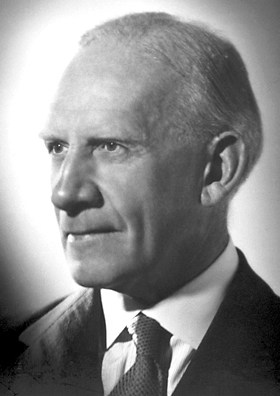
\includegraphics[width=\linewidth]{images/book3/robinson.jpg}
\end{minipage}\hfill
\begin{minipage}[t]{0.78\linewidth}
\vspace{0pt}
Robert Robinson and William Rapson published the ring-forming sequence in 1935, in work aimed at the
synthesis of steroids. Robinson's main achievements were the structures and syntheses of alkaloids,
for which he received the 1947 Nobel Prize in Chemistry. In 1950 Peter Wieland and Karl Miescher made
the bicyclic diketone of this chapter's problem, which became a common starting point for steroid and
terpene syntheses. (Portrait: unknown author, public domain; Wikimedia Commons.)
\end{minipage}
\end{history}

\begin{safety}{\ghs[5mm]{GHS02}\,\ghs[5mm]{GHS05}\,\ghs[5mm]{GHS06}\,\ghs[5mm]{GHS07}\,\ghs[5mm]{GHS08}\,\ghs[5mm]{GHS09}}
But-3-en-2-one is flammable, very toxic, corrosive and hazardous to the aquatic environment, and a powerful lachrymator; it is handled only
in a fume hood. Cyclohex-2-en-1-one is flammable and toxic. Organolithiums, Grignard reagents and
cuprates react violently with water and are handled under inert gas.
% ledger: ghs:MVK, ghs:cyclohexenone, ghs:MeMgBr
\end{safety}

\section{Exercises}

\begin{exercise}[$\star$]\label{exo:b2:conjugate-additions:1}
Predict 1,2- or 1,4-addition to cyclohex-2-en-1-one for: \ce{CH3MgBr}; \ce{(CH3)2CuLi};
\ce{C6H5SH} with a little base; \ce{LiAlH4}.
\end{exercise}

\begin{exercise}[$\star$]\label{exo:b2:conjugate-additions:2}
Classify as \omterm{def:b2:conjugate-additions:michael}{Michael donor} or \omterm{def:b2:conjugate-additions:michael}{Michael acceptor}: pentane-2,4-dione, propenenitrile \ce{CH2=CHCN},
nitromethane, methyl propenoate, diethyl propanedioate, but-3-en-2-one.
\end{exercise}

\begin{exercise}[$\star$]\label{exo:b2:conjugate-additions:3}
Write the preparation of lithium dibutylcuprate from 1-bromobutane, lithium and copper(I) iodide.
\end{exercise}

\begin{exercise}[$\star$]\label{exo:b2:conjugate-additions:4}
Give the product of diethyl propanedioate with but-3-en-2-one and a catalytic amount of sodium
ethoxide, then the product after hydrolysis and heating.
\end{exercise}

\begin{exercise}[$\star\star$]\label{exo:b2:conjugate-additions:5}
Propose a preparation of 3-methylcyclohexanone from cyclohex-2-en-1-one, and explain why
methylmagnesium bromide would be a poor choice.
\end{exercise}

\begin{exercise}[$\star\star$]\label{exo:b2:conjugate-additions:6}
Ethanethiol adds to but-3-en-2-one with a trace of triethylamine. Write the mechanism and say why the
thiolate adds 1,4.
\end{exercise}

\begin{exercise}[$\star\star$]\label{exo:b2:conjugate-additions:7}
Cyanide with cyclohex-2-en-1-one gives, at low temperature and short times, the cyanohydrin; at higher
temperature and longer times, 3-oxocyclohexane-1-carbonitrile. Explain with kinetic and thermodynamic
control.
\end{exercise}

\begin{exercise}[$\star\star$]\label{exo:b2:conjugate-additions:8}
Give the \omterm{def:b2:conjugate-additions:robinson}{Robinson annulation} product of 2-methylcyclohexane-1,3-dione with but-3-en-2-one, then that
of cyclohexanone with but-3-en-2-one.
\end{exercise}

\begin{exercise}[$\star\star$]\label{exo:b2:conjugate-additions:9}
Disconnect heptane-2,6-dione into a \omterm{def:b2:conjugate-additions:michael}{Michael donor} and a \omterm{def:b2:conjugate-additions:michael}{Michael acceptor}, and propose conditions.
\end{exercise}

\begin{exercise}[$\star\star\star$]\label{exo:b2:conjugate-additions:10}
A simple \omterm{def:b2:enolates-aldol:aldol}{aldol addition} is easily reversed in base; the Michael adduct of diethyl propanedioate and
but-3-en-2-one is not. Explain with the bonds made and broken and with the acidity of the product.
\end{exercise}

\begin{exercise}[$\star\star\star$]\label{exo:b2:conjugate-additions:11}
Diethyl propanedioate with two equivalents of methyl propenoate and a catalytic base gives a product
with no remaining \ce{C-H} between its two ester groups. Draw it and explain.
\end{exercise}

\begin{exercise}[$\star\star\star$]\label{exo:b2:conjugate-additions:12}
2-Methylcyclohexanone and but-3-en-2-one in a \omterm{def:b2:conjugate-additions:robinson}{Robinson annulation} can react through either \omterm{def:b2:enolates-aldol:enolate}{enolate}.
Draw both products and say which conditions favour the one with the methyl group on the ring-fusion
carbon.
\end{exercise}

\section{Problem: The Wieland--Miescher Ketone}

\begin{problem}[{Weekend problem --- the acidic donor, the Michael adduct, the intramolecular aldol and
its dehydration, the stereocentre and the mass balance of a preparation}]
\label{pb:b2:conjugate-additions:1}
Preparation (exercise data): \qty{10.0}{g} of 2-methylcyclohexane-1,3-dione react with a slight excess
of but-3-en-2-one and a catalytic base (\omterm{def:b2:conjugate-additions:michael}{Michael addition}); the triketone is then cyclised with a
\omterm{def:b2:amines:class}{secondary amine} and an acid (\omterm{def:b2:enolates-aldol:aldol}{aldol}, dehydration). Overall yield: 70~\%. The parent cyclohexane-1,3-dione
has $\mathrm pK_a = 5.3$ in water. Molar masses (\unit{g/mol}): C 12.011, H 1.008, O 15.999.
% ledger: pka:cyclohexanedione, aw:C, aw:H, aw:O, ghs:methylcyclohexanedione, ghs:MVK

\medskip
\noindent\textbf{Part I --- The donor.}
\begin{enumerate}
  \item Draw 2-methylcyclohexane-1,3-dione and mark its most acidic hydrogen.
  \item Why is that hydrogen so much more acidic than the $\alpha$ hydrogens of cyclohexanone?
  \item Draw the three resonance structures of its \omterm{def:b2:enolates-aldol:enolate}{enolate}.
  \item Is hydroxide or ethoxide strong enough to form this \omterm{def:b2:enolates-aldol:enolate}{enolate} completely? Use the $\mathrm pK_a$.
  \item Write the \omterm{def:b2:enolates-aldol:tautomerism}{enol} of the dione that involves C2, and say why the methyl group on C2 does not
        prevent it.
  \item Is this \omterm{def:b2:enolates-aldol:enolate}{enolate} hard or soft? Which site of but-3-en-2-one will it attack?
\end{enumerate}

\medskip
\noindent\textbf{Part II --- The Michael adduct.}
\begin{enumerate}[resume]
  \item Write the \omterm{def:b2:conjugate-additions:michael}{Michael addition} and name the triketone formed.
  \item Why is only a catalytic amount of base needed?
  \item Why does the new bond form at C2 of the dione rather than at its oxygen?
  \item How many quaternary carbons does the triketone have?
  \item Identify the 1,5-dicarbonyl relationship in the triketone.
  \item Why is a slight excess of but-3-en-2-one used, and why only slight?
\end{enumerate}

\medskip
\noindent\textbf{Part III --- The ring closure.}
\begin{enumerate}[resume]
  \item List the carbons of the triketone that bear $\alpha$ hydrogens.
  \item Which \omterm{def:b2:enolates-aldol:enolate}{enolate}, attacking which carbonyl, closes a six-membered ring?
  \item Which other ring closures could be attempted, and why do they not give the product?
  \item Write the \omterm{def:b2:enolates-aldol:aldol}{aldol} formed and the dehydration that follows.
  \item Why is the dehydration easy?
  \item Name the functional groups of the Wieland--Miescher ketone.
\end{enumerate}

\medskip
\noindent\textbf{Part IV --- Stereochemistry and mass balance.}
\begin{enumerate}[resume]
  \item Which carbon of the product is a stereocentre?
  \item Is the product of this preparation optically active? Explain.
  \item Compute the molar masses of the dione, of but-3-en-2-one and of the product
        \ce{C11H14O2}.
  \item Write the overall equation and check it with the formulas.
  \item Compute the amount of dione used.
  \item State the mass of Wieland--Miescher ketone obtained at 70~\% overall yield.
\end{enumerate}
\end{problem}
